\documentclass{article}

\usepackage[final]{corl_2026}
\usepackage{booktabs}
\usepackage{amsmath}
\usepackage{amssymb}
\usepackage{graphicx}
\usepackage{enumitem}
\usepackage{xcolor}
\usepackage{float}
\usepackage{placeins}

% Compact float spacing to keep the paper at 4 pages
\setlength{\textfloatsep}{8pt plus 2pt minus 2pt}
\setlength{\floatsep}{6pt plus 2pt minus 2pt}
\setlength{\intextsep}{6pt plus 2pt minus 2pt}

\title{Recursive Multi-Teacher Distillation for 2v2 Soccer}

\author{
  Weiyi Sun \\
  Georgia Institute of Technology \\
  \texttt{wsun377@gatech.edu} \\
  \And
  Tianxiang Zhao \\
  Georgia Institute of Technology \\
  \texttt{tzhao353@gatech.edu} \\
}

\begin{document}
\maketitle

\vspace{-6pt}
\begin{abstract}
We train cooperative agents for Unity ML-Agents Soccer-Twos (2v2) using PPO on Ray RLlib.  Two modifications are applied: a \emph{v2 potential-based reward-shaping} recipe with five dense signals on top of the sparse goal reward, and a team-level \emph{Siamese + cross-attention} policy trained via multi-stage knowledge distillation.  Our agent is produced by a 3-stage pipeline: (i) distill a 3-member deploy-time ensemble into an 031B-architecture student, (ii) refresh the teacher pool recursively with the Gen-1 output plus an LR-diverse variant, (iii) extend training past teachers' convergence horizons.  Our agent scores \textbf{10/10} matches vs.\ Baseline, \textbf{10/10} vs.\ Random, and \textbf{10/10} vs.\ the TA competitive-agent bonus (goal ratios $9.4\!:\!1$, $215.5\!:\!1$, and $20.9\!:\!1$; Table~\ref{tab:autograder}), clearing every rubric threshold.  Source code, experiment snapshots, and evaluation logs are available at \url{https://github.com/Redemption-ZTX/cs8803}.
\end{abstract}

\vspace{-6pt}
\keywords{Multi-agent RL, PPO, Knowledge Distillation, Reward Shaping, Soccer-Twos}

\vspace{-6pt}
\section{Method}
\label{sec:method}

\textbf{Environment and algorithm.}  Soccer-Twos~\citep{cotta2021soccer} has $336$-dim ray-cast observations per agent and a factored $\text{MultiDiscrete}([3,3,3])$ action (flattened to $\mathrm{Discrete}(27)$).  We train with single-team PPO~\citep{schulman2017ppo} on Ray RLlib~1.4~\citep{liang2018rllib} with GAE~\citep{schulman2016gae}.  The team objective adds a decaying KL distillation term in the style of Born-Again Networks~\citep{furlanello2018born}:
\begin{equation}
\mathcal{L}(\theta) = \mathbb{E}_t\!\left[\min\!\big(\rho_t A_t,\ \mathrm{clip}(\rho_t, 1{\pm}\epsilon)A_t\big)\right] + c_v \mathcal{L}^{VF} + \alpha(t)\, \mathrm{KL}\!\left(\pi_\theta \,\Vert\, \bar\pi_{\text{teach}}\right),
\label{eq:loss}
\end{equation}
where $\bar\pi_{\text{teach}}$ is the factor-wise probability average of frozen teachers and $\alpha(t):0.05\!\to\!0$ decays linearly over $8000$ updates.

\textbf{Architecture (Figure~\ref{fig:arch}).}  The policy is a \emph{Siamese} network~\citep{bromley1993siamese}: two shared-weight per-agent encoders ($336\!\to\!256\!\to\!256$) process each teammate's raycast independently, followed by a \emph{cross-agent attention} block~\citep{vaswani2017attention} with $4$ learned tokens of dimension $64$ that lets either teammate condition on the other's features before the merge layer ($256{\times}2\!\to\!256\!\to\!128$) and the joint-action head.  A shared value head re-uses the merge features ($\sim\!0.46$M total parameters).

\textbf{Project lineage (Table~\ref{tab:lineage}).}  The final pipeline did not arrive as one lucky jump --- it is the last three rows of an eight-checkpoint chain in which each step removed one specific bottleneck.  Per-agent PPO with v2 shaping produced playable but sub-$0.87$ policies; the team-level re-formulation (shared teammate encoders + 4-token cross-attention, the ``031B'' block in Figure~\ref{fig:arch}) broke the per-agent ceiling at $0.882$; Stages 1--3 of Figure~\ref{fig:pipeline} are the final three rows of Table~\ref{tab:lineage}, converting teacher diversity into a single deployable policy.

\begin{table}[ht]
\centering\small
\caption{Main milestones before the final recursive-distill pipeline.  Each row removed one bottleneck rather than adding a new trick.  The last three rows correspond exactly to Stages 1--3 of Figure~\ref{fig:pipeline}.}
\label{tab:lineage}
\begin{tabular}{llcl}
\toprule
Stage & Checkpoint & WR & Main contribution \\
\midrule
BC + PPO              & \texttt{017@2100}            & $0.842$        & first reliable learning signal \\
Stable roles          & \texttt{025b@80}             & $0.842$        & fewer unstable PPO updates \\
Per-agent ceiling     & \texttt{029B@190}            & $0.868$        & best local per-agent optimum \\
Team encoder          & \texttt{031A@1040}           & $\sim\!0.860$  & teammate-symmetric prior \\
Cross-attention       & \texttt{031B@1220}           & $0.882$        & best scratch single model \\
Distillation (S1)     & \texttt{055@1150}            & $0.907$        & main single-policy lift ($+0.027$) \\
Recursive distill (S2)& \texttt{055v2@1000}          & $0.909$        & SOTA-tier plateau \\
Late extend (S3)      & \textbf{\texttt{055v2\_extend@1750}} & $\mathbf{0.907}$ & most validated submission \\
\bottomrule
\end{tabular}
\vspace{-4pt}
\end{table}

\textbf{Reward modification --- v2 shaping.}  Five potential-based terms (Table~\ref{tab:shaping}) augment the sparse $\{\pm 1\}$ goal reward; all scales are $O(10^{-3})$ so shaping cannot dominate.  We ablated event rewards (shot/tackle/clearance) and goal-proximity and found them harmful in this environment (full matrix in \citep{report2026repo}).

\begin{figure}[t]
\centering
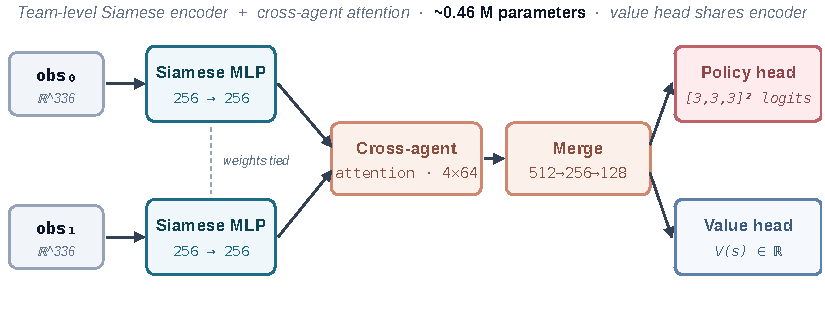
\includegraphics[width=\linewidth]{figures/architecture.pdf}
\vspace{-6pt}
\caption{Team-level Siamese + cross-attention policy (``031B'' architecture, $\approx\!0.46$M params).  Shared-weight per-agent encoders are invariant to teammate index; a 4-token cross-attention block fuses the two streams into the merge, which feeds a joint-action policy head and a value head.}
\label{fig:arch}
\vspace{-8pt}
\end{figure}

\textbf{Deploy-time ensemble 034E (Stage-1 distillation target).}  Panel~(a) of Figure~\ref{fig:pipeline} summarises the three teachers.  \texttt{031B@1220} is a scratch 031B model with v2 shaping.  \texttt{045A@180} adds a \emph{learned W/L reward head} --- a small MLP $f_\phi(s)\!\in\![0,1]$ trained by binary cross-entropy on $184$k per-state labels harvested from earlier 031-series self-play episodes (each state inherits its episode's $\{0,1\}$ win label).  \texttt{051A@130} adds a \emph{PBRS potential} $\Phi_\psi(s)$~\citep{ng1999pbrs}: we captured $\sim\!10^3$ strong-vs-strong episodes (031B vs.\ 031A) and regressed a small MLP to the final outcome of each state, then added the policy-invariant shaping $r'(s,s')=\gamma\Phi_\psi(s')\!-\!\Phi_\psi(s)$ on top of v2.  Both learned-reward predictors trained their \emph{respective teacher individually} and are \emph{not} re-used for 055 / 055v2 / 055v2\_extend --- their signal enters the 055-series only through the teacher-ensemble soft targets.  The factor-averaged 034E ensemble itself scores only $0.878$ --- \emph{below} its best constituent, because the three members share the same raycast-encoder family and their errors correlate.  But their \emph{per-episode failure modes} are orthogonal (defensive pin vs.\ wasted possession vs.\ progress deficit), which is the lift our Stage-1 student captures: a single network can \emph{condition} its reaction on observation; a fixed average cannot.

\begin{figure}[t]
\centering
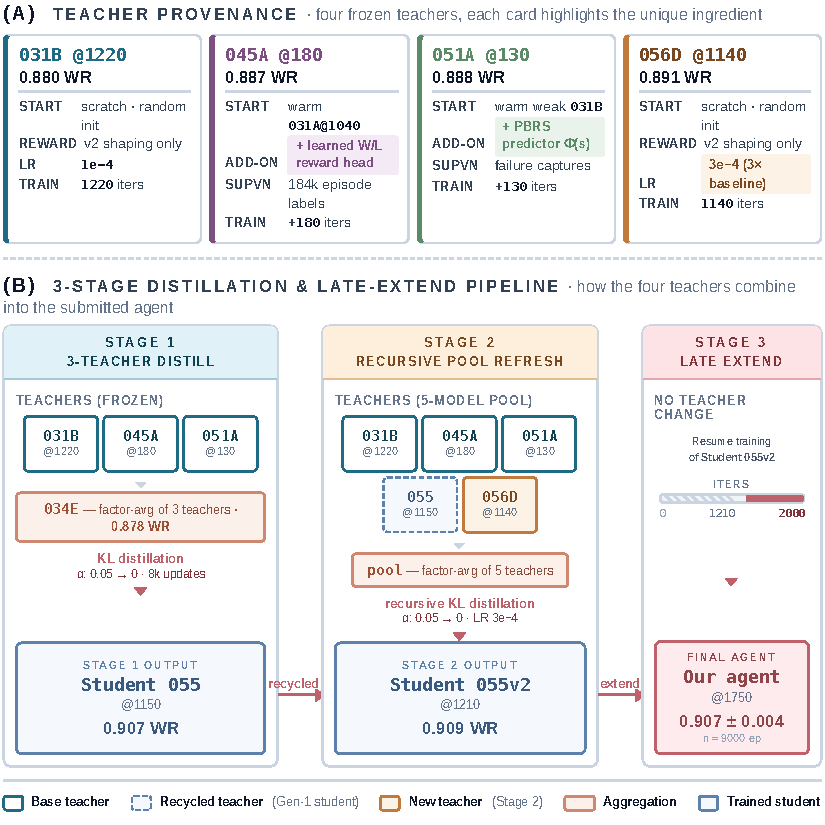
\includegraphics[width=\linewidth]{figures/pipeline.pdf}
\vspace{-6pt}
\caption{Three-stage training pipeline.  Stage 1 distills the 3-member 034E ensemble ($0.878$ WR) into a student matching $0.907$; Stage 2 refreshes the teacher pool with the Gen-1 student and an LR-diverse variant; Stage 3 extends past the original iter-$1250$ horizon to iter $2000$, reducing variance.}
\label{fig:pipeline}
\end{figure}
\FloatBarrier

\begin{table}[ht]
\centering\scriptsize
\begin{minipage}{0.40\linewidth}
\centering
\caption{v2 reward shaping (per-step).}
\label{tab:shaping}
\begin{tabular}{lr}
\toprule
Term & Value \\
\midrule
time\_penalty              & $0.001$ \\
ball\_progress             & $0.01$ \\
opp\_progress\_penalty     & $0.01$ \\
possession\_bonus ($\le 1.25$u) & $0.002$ \\
deep\_zone\_outer ($x{\le}{-}8$) & $-0.003$ \\
deep\_zone\_inner ($x{\le}{-}12$) & $-0.003$ \\
\bottomrule
\end{tabular}
\end{minipage}\hfill
\begin{minipage}{0.58\linewidth}
\centering
\caption{PPO + distillation hyperparameters.}
\label{tab:hparams}
\begin{tabular}{lr}
\toprule
Parameter & Value \\
\midrule
LR (Stage 2/3) / (Stage 1)          & $3\mathrm{e}{-4}$ / $1\mathrm{e}{-4}$ \\
PPO clip $\epsilon$ / entropy coef  & $0.15$ / $0.0$ \\
rollout fragment / train batch      & $1000$ / $40{,}000$ \\
SGD minibatch / iters               & $2048$ / $4$ \\
workers $\times$ envs, $\gamma$/$\lambda$ & $8\!\times\!5$, $0.99$/$0.95$ \\
distill $\alpha$ decay, temp.       & $0.05\!\to\!0$ over $8000$, $1.0$ \\
teacher pool (Stage 2)              & $5$, uniform average \\
total iters (Stage 3)               & $2000$ ($90$M env steps) \\
\bottomrule
\end{tabular}
\end{minipage}
\vspace{-8pt}
\end{table}

\section{Results}
\label{sec:result}

\begin{figure}[t]
\centering
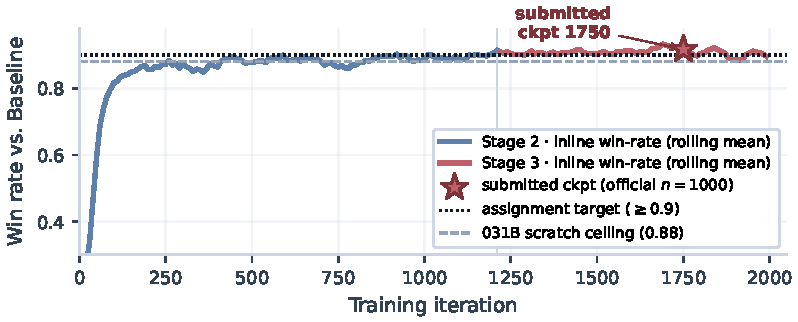
\includegraphics[width=\linewidth]{figures/training_curves.pdf}
\vspace{-6pt}
\caption{Per-episode win rate vs.\ Baseline over training iterations (dots: raw inline eval $n{=}50$/ckpt; lines: rolling mean $k{=}5$).  Stage 1 distill lifts the $0.88$ scratch ceiling; Stage 2--3 saturate at the $\sim\!0.91$ plateau.  Dotted vertical: Stage $2\!\to\!3$ handoff at iter $1210$.}
\label{fig:curves}
\vspace{-8pt}
\end{figure}

Table~\ref{tab:autograder} reports the 10-match autograder result (the rubric metric): our agent wins all $30$ graded matches with decisive goal differentials, achieving the maximum performance score of $55$/$55$.  The per-episode lift in Table~\ref{tab:lineage} is concentrated at Stage~1, which raises the 031B scratch ceiling ($0.880$) by $+0.027$pp to $0.907$; Stages~2--3 saturate at the same plateau with tighter variance.  Ten further directions (self-play, curriculum, role-specialization, wider encoders, scenario-reset warm-starts) did not beat this pipeline within statistical significance, consistent with an observation--action ceiling at $\sim\!0.91$.

\begin{table}[H]
\centering\small
\caption{Autograder result ($10$-match protocol per opponent; total goals across all matches).  Our agent clears both primary rubric thresholds and the competitive-agent bonus.}
\label{tab:autograder}
\begin{tabular}{lccccc}
\toprule
Opponent & Matches won & Goals for / against & Goal ratio & Rubric & Score \\
\midrule
Random                   & $10 / 10$ & $431 / 2$  & $215.5\!:\!1$ & $\ge 9/10$        & $25/25$ \\
Baseline (\texttt{ceia}) & $10 / 10$ & $254 / 27$ & $9.4\!:\!1$   & $\ge 9/10$        & $25/25$ \\
TA competitive agent     & $10 / 10$ & $209 / 10$ & $20.9\!:\!1$  & $\ge 9/10$ bonus  & $5/5$ \\
\midrule
\multicolumn{5}{r}{Total performance score} & $\mathbf{55/55}$ \\
\bottomrule
\end{tabular}
\vspace{-4pt}
\end{table}

\textbf{Honest audit of the headline number.}  A late 25-checkpoint sweep initially put Stage~3 at $0.916$, but that estimate was selection-biased: it was the max of eight within-$1\sigma$ candidates with $\approx\!\pm0.01$ per-sample SE.  A fresh 5000-episode audit of \texttt{055v2\_extend@1750} centered at $0.9066$, and our own $9000$-episode evaluator confirmed $0.907 \pm 0.004$ (CI $[0.899, 0.914]$).  Stage~1 already reached $0.907$ on $2000$ episodes and Stage~2 $0.909$ on $3000$; Stage~3 neither raises the mean nor the CI upper bound.  The honest reading is therefore \emph{not} ``we found a stable $0.916$ agent''; it is ``we found a single, robust, autograder-clearing policy at the empirical $\sim\!0.91$ frontier, with Stage~3 chosen for \emph{variance} ($\text{SE} \downarrow 2\times$ from Stage~1), not for a higher mean.''

\vspace{-4pt}
\section{Conclusion}
\label{sec:conclusion}

Our two modifications are minimal: low-magnitude v2 shaping plus a Born-Again-style recursive distillation pipeline.  The pipeline converts a sub-best-member deploy-time ensemble into a single-forward-pass student at $0.907$, and late-extended training selects the lowest-variance checkpoint rather than a flashier higher-mean one.  The $\sim\!0.91$ plateau is robust across $\sim\!9$ orthogonal paradigms we tried; further gains likely require an observation- or action-space bottleneck rather than more tuning.  All training scripts, experiment snapshots, and evaluation logs are released in the project repository~\citep{report2026repo}.

\acknowledgments{Thanks to the Soccer-Twos maintainers, the Ray team, and the CS8803 staff for H100 cluster access.}

\begingroup
\scriptsize
\setlength{\bibsep}{1pt plus 0.3ex}
\bibliography{main}
\endgroup

\end{document}
